\documentclass[10pt]{article}
\usepackage[margin=0.85in]{geometry}
\usepackage{amsmath,amssymb,bm}
\usepackage{booktabs}
\usepackage{graphicx}
\usepackage{enumitem}
\usepackage[hidelinks]{hyperref}
\usepackage{caption}
\usepackage{titlesec}
\titlespacing*{\section}{0pt}{10pt}{4pt}
\titlespacing*{\subsection}{0pt}{8pt}{3pt}
\captionsetup{font=small,labelfont=bf,skip=4pt}
\setlist{itemsep=2pt,topsep=3pt,leftmargin=1.4em}
\setlength{\parskip}{2pt}
\newcommand{\Tr}{\mathrm{Tr}}
\newcommand{\gl}{\mathfrak{gl}}
\newcommand{\su}{\mathfrak{su}}
\newcommand{\g}{\mathfrak{g}}
\newcommand{\h}{\mathfrak{h}}
\newcommand{\n}{\mathfrak{n}}
\newcommand{\Wg}{\mathcal{W}}
\newcommand{\Alt}{\mathrm{Alt}}
\title{\vspace{-1.5cm}\Large\textbf{Fermionic Matrix Models, Fortuity, and SYK}\vspace{-6pt}}
\author{}
\date{}

\begin{document}
\maketitle
\vspace{-1.0cm}
\begin{center}\begin{minipage}{0.95\textwidth}\small
\textbf{Abstract.} We study a three-parameter family of purely fermionic quantum mechanics: $p$ flavours of
adjoint matter for a gauge algebra of rank $r$, with a nilpotent supercharge of odd degree $q$ built from traces.
The family contains $\mathcal N=2$ SYK as its rank-one member, since at $N=1$ the trace is the identity map and
$Q$ becomes a generic $q$-fermion supercharge on $p$ modes, an identification we verify numerically. The BPS
states are the cohomology of multiplication by a fixed $q$-form, and the width of the R-charge window they
occupy is set by the rank: $W=r(w_s-1)+1$ at the maximal weight, where $w_s$ is the width contributed by a
single Cartan site. R-charge concentration requires $W\le q$, hence $r(w_s-1)\le q-1$, and the measured floor
$\min_p w_s=q-1$ leaves rank $2$ at $q=3$ and rank $1$, meaning SYK, for every $q\ge5$; the cubic supercharge is
the only degree admitting a gauge group at all. The mechanism is the Weyl group. At the maximal weight the
complex is the Cartan sector carrying a $q$-form that gauge invariance forces to be Weyl invariant, and while
generic $q$-forms have bounded window, Weyl invariant ones do not: holding the Cartan at twelve modes and
varying only the Weyl group gives $W=3,3,5,5,11$ for $|\Wg|=1,2,6,24,720$. The window sees membership in this
symmetry class and nothing finer, so multi-trace couplings, which make the Cartan interaction far denser, leave
$W$ unchanged. If $-1$ lies in the Weyl group, as for $B$, $C$, $D_{\rm even}$ and most exceptional algebras, the
Cartan form vanishes and the window is maximal, so the unitary series is already optimal. Fortuity runs the
opposite way and is total: an embedded BPS state is never closed at the next rank, so no class is monotone.
\end{minipage}\end{center}
\vspace{8pt}

\section{One family}\label{sec:family}

Let $\g$ be a reductive Lie algebra of rank $r$ with a fixed invariant form, and let $\Psi^a$, $a=1,\dots,p$, be
complex fermions valued in $\g$. For $\g=\gl(N)$ we write $\Psi^a_{ij}$ with $i,j=1,\dots,N$ and
$\{\Psi^a_{ij},\bar\Psi^b_{kl}\}=\delta^{ab}\delta_{il}\delta_{jk}$, the gauge group acting by conjugation. The
Fock space is the exterior algebra
\begin{equation}
\mathcal H=\Lambda^\bullet V,\qquad V=\mathbb C^p\otimes\g,\qquad n\equiv\dim V=p\dim\g ,
\end{equation}
graded by the R-charge $k=N_\Psi=\Tr\Psi^a\bar\Psi^a$, so $\Lambda^kV$ is the $k$-fermion sector. A basis vector
of $V$ is a \emph{mode}; a basis vector of $\Lambda^kV$ is a set $S$ of $k$ modes, written $m_S$. All dynamics
comes from one supercharge,
\begin{equation}
Q=\sum_{a_1\dots a_q}C_{a_1\dots a_q}\,\Tr\!\big[\Psi^{a_1}\cdots\Psi^{a_q}\big],\qquad H=\{Q,\bar Q\}\ \ge0,
\qquad [N_\Psi,Q]=q\,Q .
\label{eq:Q}
\end{equation}
Only odd $q$ is admissible, for two independent reasons: a cyclic shift inside $\Tr[\Psi^q]$ costs $(-1)^{q-1}$,
so the trace vanishes identically for even $q$; and $Q^2=0$ needs the exchange of the two $q$-tuples in
$C\otimes C$, a permutation of $2q$ fermions built from $q^2$ transpositions, to produce a relative sign, which
again happens exactly for odd $q$.

Since every $\Psi$ is a creation operator, $Q$ contains no annihilators and acts on $\Lambda^\bullet V$ as plain
left multiplication,
\begin{equation}
Q=\omega\wedge-\,,\qquad \omega=\sum C_{a_1\dots a_q}\Tr[\Psi^{a_1}\cdots\Psi^{a_q}]\in\Lambda^qV ,
\qquad H^\bullet=\operatorname{Ann}(\omega)/(\omega).
\label{eq:wedge}
\end{equation}
The whole problem is the cohomology of multiplication by one specific element of $\Lambda^qV$. Note also that
$\omega\wedge\omega=0$ automatically for odd $q$, so nilpotency survives any modification of the couplings or of
the index structure, a fact we use freely in \S\ref{sec:weyl}.

\subsection{SYK is the member at $N=1$}

The family is usually presented as a matrix generalisation of SYK, but SYK is already inside it. At $N=1$ the
matrices are $1\times1$, the trace is the identity map, and \eqref{eq:Q} reads
\begin{equation}
Q=C_{a_1\dots a_q}\,\psi^{a_1}\cdots\psi^{a_q},
\end{equation}
which is $\mathcal N=2$ SYK with $n=p$ complex fermions. The gauge algebra is $u(1)$, whose adjoint action is
trivial, so no constraint whatever is placed on $C$; this is why the SYK coupling is free while the matrix
coupling is not. Randomness plays no role in what follows. What a Gaussian ensemble supplies is genericity, and
genericity is optimal here for a structural reason: matrix ranks are lower semicontinuous in $\omega$, so
specialising the couplings can only enlarge the cohomology.

We checked the identification rather than assuming it, by running the full matrix machinery (weight
decomposition, trace-structured $\omega$, exact integer ranks) at $N=1$ and comparing against a bare generic
$q$-form. The two agree for every $p$ from $4$ to $12$, giving in both cases $W=3,4,3,2$ as $p\equiv0,1,2,3$
mod $4$, with identical Betti numbers.

What varies along the family is therefore not the coupling tensor but the \emph{interaction hypergraph}. Call a
\emph{triangle} the support of a non-zero term of $\omega$, a set of $q$ distinct modes. SYK has every one of the
$\binom p q$ possible triangles. At general $N$ there are $pN^2$ modes but only the index-loop triangles survive,
a fraction of order $6/N^3$ for $q=3$. The parameter $N$ dials the hypergraph from complete to sparse, and the
question is what that does to the cohomology.

\subsection{What concentration asks}

The Cartan torus acts on $\Psi_{ij}$ by $u_iu_j^{-1}$, so that mode carries weight $e_i-e_j$ and a state's weight
is the row sums minus the column sums of its occupation matrix; diagonal modes carry weight zero. Since $Q$ is a
gauge singlet it preserves the weight, and since $[N_\Psi,Q]=qQ$ it raises $k$ by $q$, so the cohomology splits
into complexes labelled by $(\lambda,\omega_{\rm fl},c)$ with $\lambda$ a $U(N)$ irrep, $\omega_{\rm fl}\in\mathbb
Z_p$ a flavour charge, and $c=k\bmod q$. R-charge concentration, in the sense of Chang, Chen, Sia and Yang, says
that in each complex of macroscopic index all BPS states sit at one degree. Writing $W$ for the number of
consecutive R-charges carrying BPS states, a necessary condition is
\begin{equation}
W\ \le\ q ,
\label{eq:conc}
\end{equation}
since a window wider than the grading period must place two occupied degrees in one residue class. Everything
below is an estimate of $W$.

\subsection{Relation to prior work}

The two ends of the family are each well studied. The $N=1$ end is $\mathcal N=2$ SYK, where R-charge
concentration was formulated by Chang, Chen, Sia and Yang \cite{CCSY}; their \S5.1 also shows empirically that
making the couplings sparse destroys concentration, and their \S5.6 estimates the sparsity of the
$\mathcal N=4$ SYM supercharge as $\tilde N^{-3/2}$ with $\tilde N=N^2$, which is the same $N^{-3}$ scaling as
the adjoint hypergraph density quoted in \S\ref{sec:family}. Our \S\ref{sec:everyweight} makes that heuristic precise for these models. The window itself is set by the
symmetry class rather than by the density: the multi-trace models of \S\ref{sec:weyl} are substantially denser
than the single-trace model and have the same window.

The one-flavour end at general odd $q$ is the subject of Tierz \cite{Tierz}, who computes BPS multiplicities for
$\Tr[\Psi^q]$ at $(q,N)=(5,3),(5,4),(5,5),(7,4)$ and observes a factorisation $Z_{\rm BPS}=p^{b}x^{q_{\min}}
(1+x)^NT(x)$. That paper overlaps ours in three places, and we have used it to check and to correct what
follows. Its $(1+x)^N$ is the factor our slot factorisation produces at the maximal weight, where one flavour
admits no self-loop and $Q$ therefore vanishes; its observation that the traceless diagonal modes make the
cohomology a module over $\Lambda^\bullet(\mathbb C^{N-1})$, with freeness left open, is the same module
structure we use, and freeness is exactly what \eqref{eq:kunneth} establishes at the maximal weight and leaves
open elsewhere; and its \S6.1 measures the phenomenon this report is about, namely that at matched fermion
number SYK occupies exactly $q$ sectors and saturates the index while the matrix model occupies more and exceeds
it. As a check on both codes, our machinery reproduces its $(q,N)=(5,3)$ total exactly, $Z_{\rm BPS}=440$ with
profile $20,75,125,125,75,20$. Two corrections that paper forces on us are recorded in \S\ref{sec:rank} and
\S\ref{sec:fortuity}.

\section{The rank law}\label{sec:rank}

\subsection{The maximal weight, and why only self-loops survive}

\begin{figure}[t]\centering
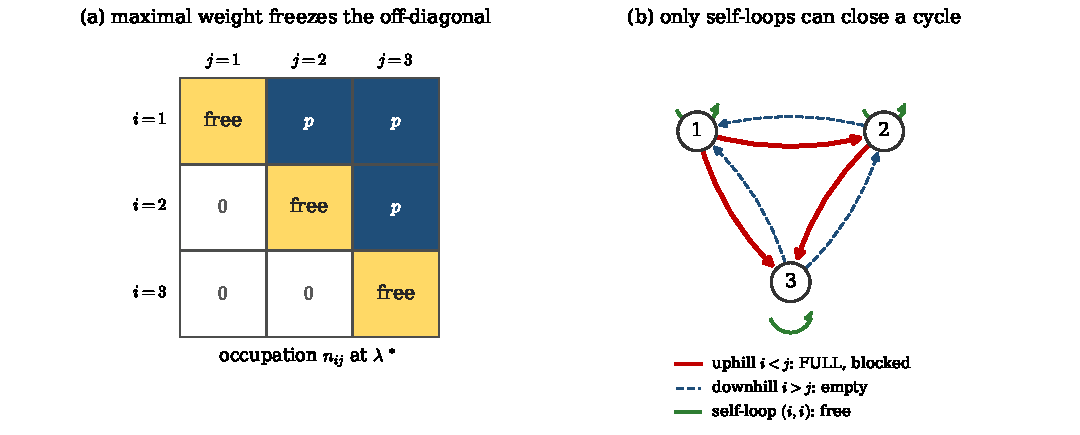
\includegraphics[width=0.93\textwidth]{report_figs/g_loops.pdf}
\caption{(a) At the maximal weight the occupation is forced: every mode with $i<j$ is full, every mode with $i>j$
is empty, and only the diagonal is free. (b) Reading modes as coloured directed edges, $Q$ creates a closed walk
$i\to j\to k\to i$ and needs all its edges empty. Uphill edges are occupied, so every creatable step is
non-increasing; a cycle of non-increasing steps must be constant, leaving only self-loops.}
\label{fig:loops}
\end{figure}

The highest weight in the Fock space is found greedily, filling row $1$ and emptying column $1$, then row $2$,
and so on, giving the fully upper-triangular occupation with
\begin{equation}
\lambda^*_i=p\,(N+1-2i),\qquad
C_2^{\max}=\tfrac12 p(p+1)\textstyle\sum_i(N+1-2i)^2=\frac{p(p+1)N(N^2-1)}{6}.
\label{eq:lamstar}
\end{equation}
At $p=1$ this is $N(N^2-1)/3$, Chen's $C_2(r_*)$, so \eqref{eq:lamstar} is its multi-flavour generalisation.
Shifting $\lambda^*$ to a partition gives row lengths $p(2N-2i)$, exactly $p$ times Chen's staircase with the
same $N-1$ non-empty rows; adding flavours stretches rows without producing new ones, a point we return to in
\S\ref{sec:fortuity}.

At $\lambda^*$ the off-diagonal sector is rigid, every upper mode occupied and every lower mode empty
(Fig.~\ref{fig:loops}a), so the weight space is an exterior algebra on the zero-weight modes,
$(\Lambda V)_{\lambda^*}\cong\Lambda^\bullet(\mathcal Z)$ with $\mathcal Z=\h\otimes\mathbb C^p$ of dimension
$pr$. Which terms of $Q$ survive is best seen graphically. Read a mode $\Psi^a_{ij}$ as a directed edge $i\to j$
of colour $a$. A term is a trace, so the $q$ modes it creates form a closed walk, and Pauli exclusion lets it act
only if every edge of that walk is empty. At the maximal weight the empty modes are precisely those with $i>j$,
together with whatever diagonal flavours remain free, so every step of a creatable walk satisfies $i_t\ge
i_{t+1}$: the walk may descend or stay level but never climb, since all uphill edges are occupied. Closing it
forces $i_1=\dots=i_q$. Only self-loops survive, meaning $q$ diagonal modes of distinct flavours at a single
site. We checked this exhaustively at $N=3$, $p=3$, where all $192$ non-zero actions of $Q$ on the maximal-weight
space are of exactly this form.

\subsection{Factorisation}

Because every surviving term sits at one site, $Q=\sum_{i=1}^r Q_i$ with $Q_i$ acting inside site $i$'s flavour
space, and since the $q$ creation operators anticommute only the totally antisymmetric part of the coupling
survives: $Q_i=\omega_{\rm sl}\wedge-$ on $\Lambda^\bullet\mathbb C^p$ with $\omega_{\rm sl}=\Alt(C)$. The $Q_i$
act on disjoint tensor factors of $\Lambda(\mathcal Z)=(\Lambda^\bullet\mathbb C^p)^{\otimes r}$, so K\"unneth
applies and Poincar\'e polynomials multiply,
\begin{equation}
Z_{\max}(t)=t^{k_0}\big(z_{\rm slot}(t)\big)^{r},\qquad
z_{\rm slot}(t)=\sum_j\dim H^j\big(\Lambda^\bullet\mathbb C^p,\ \omega_{\rm sl}\wedge\big)\,t^j ,
\label{eq:kunneth}
\end{equation}
with $k_0=p|\Delta^+|$ counting the frozen off-diagonal modes. Multiplying $r$ copies of a polynomial adds their
degree spans, so if $z_{\rm slot}$ is supported on $w_s$ degrees then
\begin{equation}
W=r\,(w_s-1)+1 .
\label{eq:ranklaw}
\end{equation}
This is the rank law. It is worth running once. At $p=q=3$ and $N=3$, the slot algebra $\Lambda^\bullet\mathbb
C^3$ has dimensions $1,3,3,1$, and $\Alt(C)$ spans the one-dimensional $\Lambda^3\mathbb C^3$, so $\omega_{\rm
sl}\wedge$ is non-zero only as $\Lambda^0\to\Lambda^3$. Hence $H^0=0$ by injectivity, $H^1=H^2=3$ because the
differential neither enters nor leaves, and $H^3=1-1=0$, giving $z_{\rm slot}=3t(1+t)$. Cubing and restoring the
prefactor yields $Z_{\max}=27t^{12}+81t^{13}+81t^{14}+27t^{15}$, in exact agreement with the computed spectrum
(Table~\ref{tab:profiles}).

\begin{table}[t]\centering\small
\begin{tabular}{llrl}
\toprule
$N$ & window ($N_\Psi$) & $W$ & BPS multiplets $h^k$\\
\midrule
2 & $5,6,7$ & 3 & $9,\ 18,\ 9$\\
3 & $12,\dots,15$ & 4 & $27,\ 81,\ 81,\ 27$\\
4 & $22,\dots,26$ & 5 & $81,\ 324,\ 486,\ 324,\ 81$\\
5 & $35,\dots,40$ & 6 & $243,\ 1215,\ 2430,\ 2430,\ 1215,\ 243$\\
\bottomrule
\end{tabular}
\caption{Exact BPS multiplets of the maximal irrep at $p=q=3$, as predicted by \eqref{eq:kunneth}: $3^N\binom Nj$
over $N+1$ consecutive charges centred on $pN^2/2$, totalling $6^N$. The factor $(1+t)^N$ is the same one that
appears in Chen's single-matrix $Z_{\rm BPS}$.}
\label{tab:profiles}
\end{table}

\subsection{SYK sits at $r=1$}

Setting $r=1$ in \eqref{eq:ranklaw} gives $W=w_s$, and $r=1$ is exactly the $N=1$ member, so the rank law already
contains SYK. This is not a coincidence of notation: $z_{\rm slot}$ is by definition the cohomology of a generic
$q$-form on $\mathbb C^p$, which is the SYK computation. The single formula therefore covers both ends of the
family, and concentration \eqref{eq:conc} becomes a condition on the rank,
\begin{equation}
r\,(w_s-1)\ \le\ q-1 .
\label{eq:conc-rank}
\end{equation}
Table~\ref{tab:rank} collects every model we have measured. The width is $r+1$ throughout, including SYK. That
$u(2)$ and $\su(3)$, different algebras of different $N$ and different dimension, give the same $W$ is a
non-trivial check that rank rather than $N$ or $\dim\g$ is the governing variable.

\begin{table}[t]\centering\small
\begin{tabular}{lccll}
\toprule
model ($p=3$, $q=3$) & rank $r$ & $W$ & $W\le q$? & evidence\\
\midrule
SYK $=u(1)$, any $p$ & 1 & 2 & yes & all $p$ from 4 to 12, matched against the matrix code\\
$u(2)$ & 2 & 3 & yes & complete spectrum, all four irreps give $9,18,9$\\
$\su(3)$ & 2 & 3 & yes & maximal weight\\
$u(3)$ & 3 & 4 & no & complete Casimir tiers $48$ down to $24$, all 13 irreps\\
$\su(4)$ & 3 & 4 & no & maximal weight\\
$u(4)$ & 4 & 5 & no & 13 irreps down to $C_2=107$\\
$\su(5)$ & 4 & 5 & no & maximal weight\\
$u(5)$ & 5 & 6 & no & maximal weight\\
\bottomrule
\end{tabular}
\caption{The rank law in measured form: $W=r+1$ across every model computed, with SYK the rank-one case.
Concentration survives exactly to rank $2$.}
\label{tab:rank}
\end{table}

\subsection{How small can $w_s$ be, and why $q=3$ is forced}

\begin{figure}[t]\centering
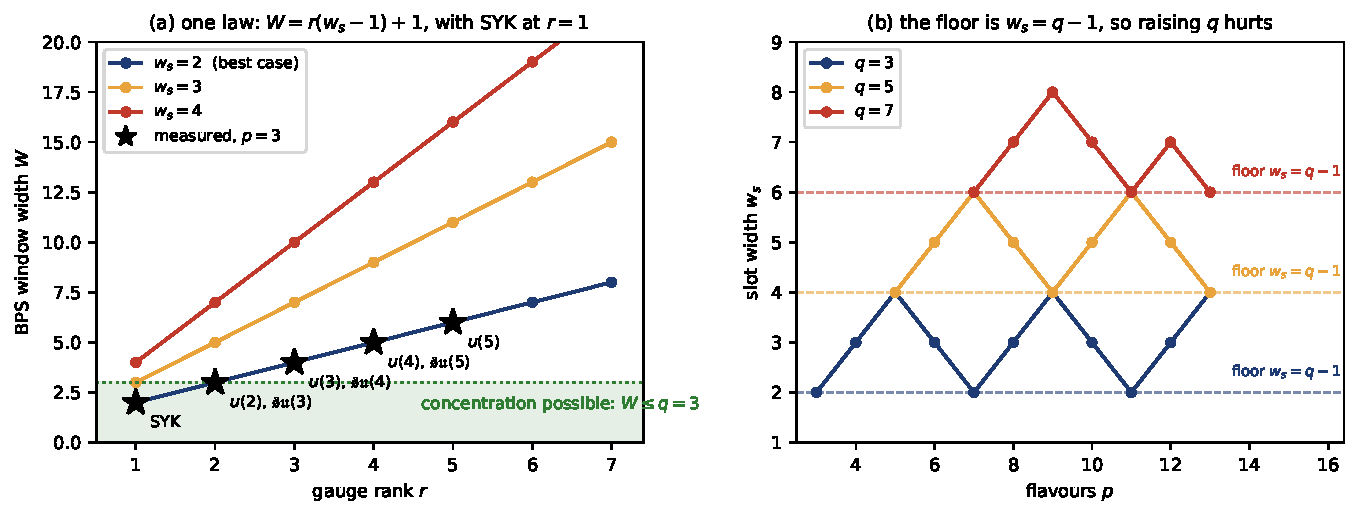
\includegraphics[width=0.95\textwidth]{report_figs/g_rank.pdf}
\caption{(a) The rank law with the measured models on it. SYK is not a separate case but the point $r=1$.
(b) The slot width for generic couplings. Its floor over $p$ is $w_s=q-1$, so larger $q$ raises the slope of the
rank law faster than it raises the ceiling $q$.}
\label{fig:rank}
\end{figure}

Everything now turns on $w_s$, and a short argument shows it can never be $1$. Grade $\Lambda^\bullet\mathbb C^p$
by $j$ mod $q$ and let $E_c=\sum_{j\equiv c}(-1)^j\binom pj$ be the Euler characteristic of class $c$; wherever
$E_c\ne0$ there must be cohomology in that class. Now $\sum_cE_c=(1-1)^p=0$, so exactly one non-zero $E_c$ is
impossible, while with $\zeta=e^{2\pi i/q}$ one has $E_c=\frac1q\sum_{m=1}^{q-1}\zeta^{-mc}(1-\zeta^m)^p$ with
every $1-\zeta^m\ne0$, so they cannot all vanish. At least two classes carry cohomology, giving $w_s\ge2$ and
hence $W\ge r+1$ at the maximal weight: concentration already requires $r\le q-1$, independently of the flavour
content.

The measured values are stronger than this bound. Computing $z_{\rm slot}$ for generic couplings gives, for
$q=3$, the sequence $w_s=2,3,4,3,2,3,4,3,2,3,4$ as $p$ runs from $3$ to $13$, and the analogous scans at $q=5$
and $q=7$ give floors of $4$ and $6$ (Fig.~\ref{fig:rank}b). In every case
\begin{equation}
\min_p w_s\ =\ q-1 ,
\label{eq:floor}
\end{equation}
so the best achievable rank law is $W=r(q-2)+1$ and the condition \eqref{eq:conc-rank} becomes $r\le
(q-1)/(q-2)$. The consequence is sharp and slightly surprising: raising $q$ makes matters worse, because it
raises the slope of the rank law faster than it raises the ceiling.

\begin{center}\small
\begin{tabular}{ccc}
\toprule
$q$ & best $w_s$ & largest rank admitting concentration\\
\midrule
3 & 2 & $2$\\
5 & 4 & $1$, that is, SYK only\\
7 & 6 & $1$, that is, SYK only\\
\bottomrule
\end{tabular}
\end{center}

So $q=3$ is the unique degree that tolerates a gauge group at all, and even there only rank $2$. Chen's choice
of a cubic supercharge is forced rather than conventional, and the three concentrating members of the family with
a non-trivial gauge group are $u(2)$ and $\su(3)$ at $q=3$, plus SYK at any $q$.

One apparent loophole should be recorded and then closed, because closing it sharpens what the rank law may be
asked to do. The table above assumes $p\ge q$. If $p<q$ then $\Lambda^q\mathbb C^p=0$, the slot differential
dies and $z_{\rm slot}=(1+t)^p$, so $w_s=p+1$. At one flavour this gives $w_s=2$ and hence $W=r+1$ at the
maximal weight for any $q$, which we confirm at $(q,N)=(3,3),(3,4),(5,3),(5,4),(7,4)$, in every case with the
binomial profile $\binom Nj$. It is tempting to conclude that $q\ge N+1$ then satisfies \eqref{eq:conc} at every
$N$. It does not. The window of the \emph{total} cohomology is wider than the window at the maximal weight once
$q\ge5$: at $(q,N)=(5,3)$ the full Fock space carries $Z_{\rm BPS}=440$ BPS states spread over six sectors
$R=2,\dots,7$ with profile $20,75,125,125,75,20$, against a maximal-weight window of four. The residues mod $5$
are $2,3,4,0,1,2$, so $R=2$ and $R=7$ share a class and concentration fails. That total agrees exactly with the
independent computation of Tierz \cite{Tierz}, whose single-matrix $\Tr[\Psi^q]$ model is the one-flavour member
of this family at general odd $q$.

Two things follow. The loophole is closed, and more importantly the irrep-independence of the window, which we
verify at $q=3$ through the Casimir descents cited in Table~\ref{tab:rank}, is \emph{false} at $q=5$. The rank
law is therefore a statement about the maximal weight, and we use it as such: at $q=3$ the descents license
reading it as a statement about the spectrum, while at larger $q$ they do not. Since the total window is then
wider than $r+1$, the conclusion that raising $q$ hurts is reinforced rather than weakened. A further caveat
attaches to the whole maximal-weight analysis: the multiplicity $6^N$ of Table~\ref{tab:profiles} is not
macroscopic, so the complexes reached here are not yet the ones the concentration hypothesis is about.

\section{Why rank: the Weyl group}\label{sec:weyl}

The rank law says what happens. This section identifies what produces it.

\subsection{The Cartan sector carries a Weyl invariant form}

By \S\ref{sec:rank} the maximal-weight complex is the Cartan sector: $pr$ modes carrying the $q$-form
$\omega|_{\mathcal Z}$. Gauge invariance does not merely restrict $\omega$ to traces. Restricted to the Cartan it
says something sharper, namely that $\omega|_{\mathcal Z}$ is invariant under the normaliser $N(T)$, hence under
the Weyl group $\Wg=N(T)/T$, which acts on $\h$ and trivially on flavour. For $u(N)$ and $\su(N)$ that group is
$S_N$ permuting the sites.

This is the whole obstruction, and it is visible by comparison. A generic, unconstrained $q$-form on $\mathbb C^n$
has bounded window: at $q=3$ we measure $W=3,4,3,2$ according to $n\bmod4$, for every $n$ up to $13$, never
growing. That is the same computation as $z_{\rm slot}$, and it is why SYK concentrates whenever $n\not\equiv1$
mod $4$. A Weyl invariant form does not behave this way.

\begin{figure}[t]\centering
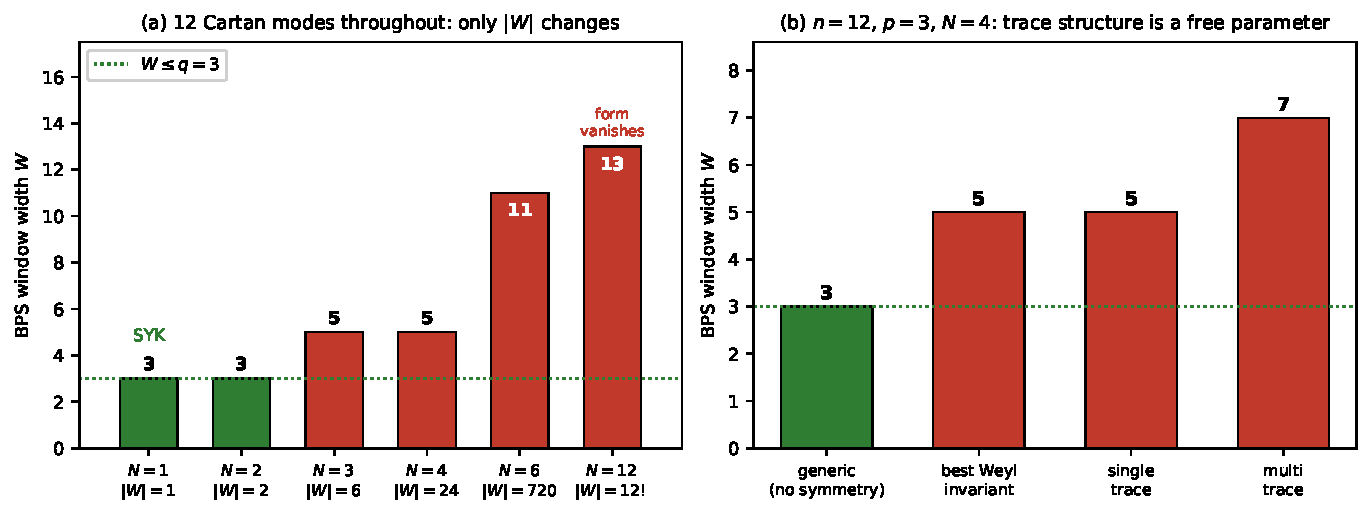
\includegraphics[width=0.95\textwidth]{report_figs/g_weyl.pdf}
\caption{(a) Twelve Cartan modes throughout, with only the Weyl group changing. Concentration survives while
$|\Wg|\le2$ and fails from $|\Wg|=6$ on. The left-hand bar is SYK. (b) At $n=12$, $p=3$, $N=4$: every Weyl invariant
coupling, whatever its trace structure or density, sits well above the generic value.}
\label{fig:weyl}
\end{figure}

The controlled experiment is to hold the Cartan size fixed and vary only the Weyl group. Taking $n=pr=12$ modes
throughout and letting $(p,N)$ range over the factorisations of $12$, so that $|\Wg|=|S_N|$ runs from $1$ to
$12!$ while nothing else changes, gives the following, each entry the narrowest window found over twenty random
draws of a generic $\Wg$-invariant form.

\begin{center}\small
\begin{tabular}{rrrl}
\toprule
$p$ & $N$ & $|\Wg|$ & narrowest $W$ over 20 draws\\
\midrule
12 & 1 & 1 & $3$ \quad(this row is SYK)\\
6 & 2 & 2 & $3$ \quad(20 of 20 draws)\\
4 & 3 & 6 & $5$ \quad(20 of 20 draws)\\
3 & 4 & 24 & $5$ \quad(19 of 20; one draw gave $7$)\\
2 & 6 & 720 & $11$\\
1 & 12 & $12!$ & the invariant form vanishes, so $W=13$\\
\bottomrule
\end{tabular}
\end{center}

The window grows monotonically with the Weyl group at fixed mode count. Since lower semicontinuity makes generic
couplings optimal, the third and fourth rows say that \emph{no} choice of gauge invariant coupling achieves $W\le
3$ at rank $3$ or more, which is the no-go in its strongest measured form.

\subsection{The window sees the symmetry class and nothing finer}

Membership in the Weyl invariant class is the whole of what the window responds to. The sharpest way to see this
is to vary the trace structure, which changes the Cartan interaction drastically while staying inside the class.
A single trace of $q$ diagonal matrices localises, $\Tr[H_1\cdots H_q]=\sum_i\prod_t(H_t)_{ii}$, so a Cartan
triangle needs $q$ distinct flavours at the \emph{same} site and the interaction is very sparse. Multi-trace
terms are equally gauge invariant and do not localise: $\Tr[\Psi^a]\Tr[\Psi^b\Psi^c]$ restricted to the Cartan is
$\sum_{i,j}\Psi^a_{ii}\Psi^b_{jj}\Psi^c_{jj}$, straddling two sites, and the triple trace straddles three. Since
$\omega\wedge\omega=0$ for any odd form, nilpotency is untouched, so these are legitimate models.

Their combinatorics is entirely different and their window is identical. Writing $\alpha_0$ for the largest
triangle-free set of Cartan modes, at $N=4$ and $p=3$:

\begin{center}\small
\begin{tabular}{lrrrr}
\toprule
trace structure & Cartan triangles & $\alpha_0$ & bound \eqref{eq:cartan} & measured $W$\\
\midrule
single only & 4 & 8 & 5 & 5\\
single $+$ double & 100 & 5 & $-1$ (vacuous) & 5\\
single $+$ double $+$ triple & 124 & 5 & $-1$ (vacuous) & 5\\
double only & 100 & 5 & $-1$ (vacuous) & 7\\
\bottomrule
\end{tabular}
\end{center}

Delocalising the Cartan interaction multiplies the triangle count by thirty and collapses $\alpha_0$ from $2N$
to $N+1$, and $W$ does not move; only the edge multiplicities thin, from $27,81,81,27$ to $11,81,81,11$ at $N=3$.
Double-trace alone is wider still. This is what the Weyl picture predicts: all of these forms lie in the class
Fig.~\ref{fig:weyl}a has already measured, and Fig.~\ref{fig:weyl}b shows each of them at or above the best value
that class allows, well away from the generic one. Density and trace structure are free parameters within the
class, and the window does not see them.

\subsection{Most gauge groups are worse, and the unitary series is optimal}

The next idea is to shop for a better gauge group, and Lie theory closes that down in one line. Suppose
$-\mathrm{id}\in\Wg$. It acts as $-1$ on every Cartan mode, hence as $(-1)^q=-1$ on a $q$-form with $q$ odd, and
$q$ must be odd. Invariance then forces $\omega|_{\mathcal Z}=0$, so $Q$ vanishes on the maximal-weight complex,
every state there is BPS, and $W=pr+1$, the widest possible value.

The Weyl groups containing $-\mathrm{id}$ are those of $B_r$, $C_r$, $D_r$ with $r$ even, $G_2$, $F_4$, $E_7$ and
$E_8$. Every orthogonal, symplectic and most exceptional gauge groups are therefore strictly worse than unitary.
Only $A_r$, $D_r$ with $r$ odd, and $E_6$ escape, and among these $\su(N)$ is what we have measured. The tempting
option of a small Weyl group, $\su(2)^r$ with $|\Wg|=2^r$, is a trap for the same reason: $(\mathbb Z_2)^r$
contains $-\mathrm{id}$, so its Cartan form vanishes identically. A Weyl group must be rich enough not to kill
the form and small enough not to constrain it, and $S_N$ with $N\le2$ is essentially the only solution.

\section{A bound valid at every weight}\label{sec:everyweight}

The rank law is derived at the maximal weight, where the rigidity of the off-diagonal sector does the work. A
weaker statement holds everywhere, by an elementary argument that is worth keeping because it is the only part of
the analysis not confined to the top of the spectrum.

Recall that a triangle is the support of a non-zero term of $\omega$. Call a set of modes $S$ \emph{critical} if
every triangle meets it partially, $0<|T\cap S|<3$ for all $T$; equivalently, neither $S$ nor its complement
contains a triangle. At $N=3$, $p=q=3$ there are $195$ triangles on $27$ modes out of $\binom{27}3=2925$ possible
triples, so the hypergraph is sparse, and criticality is easy to arrange.

\begin{figure}[t]\centering
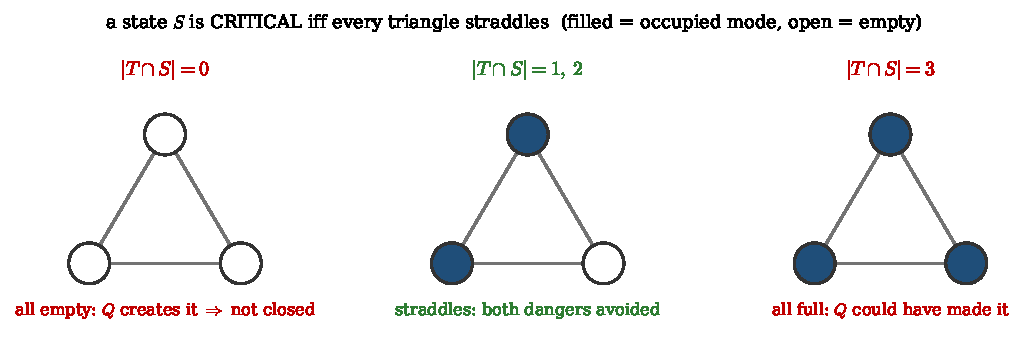
\includegraphics[width=0.93\textwidth]{report_figs/g_critical.pdf}
\caption{The three cases. If a triangle is entirely empty, $Q$ can create it and $S$ is not closed. If it is
entirely occupied, $S$ could have been produced by $Q$ and the non-exactness argument fails. Only straddling
triangles avoid both.}
\label{fig:critical}
\end{figure}

The two inequalities do different jobs. The upper one makes $m_S$ closed: for $\omega_T\wedge m_S$ to be non-zero
all $q$ modes of $T$ must be absent from $S$, which criticality excludes, so every term is Pauli-blocked. The
lower one makes $m_S$ non-exact: since $Q$ only ever adds a triangle, the coefficient of $m_S$ in $\omega\wedge
y$ is $\sum_{T\subseteq S}\pm c_T\,y_{S\setminus T}$, and criticality gives $T\not\subseteq S$ for every
triangle, so that sum is empty for every $y$ while $m_S$ has coefficient $1$ on itself. Each critical set thus
gives a non-zero class in $H^{|S|}$, and distinct ones give independent classes.

Letting $\alpha$ be the largest triangle-free set and $\tau=n-\alpha$ the transversal number, $S$ is critical
exactly when both $S$ and $S^c$ are hitting sets, so critical sets live in $\tau\le|S|\le n-\tau$ and
\begin{equation}
W\ \ge\ n-2\tau+1\ =\ 2\alpha-n+1 .
\label{eq:taubound}
\end{equation}
Wide windows are the signature of a hypergraph with large triangle-free sets.

Gauge invariance supplies such a set for free. Each term of $Q$ is a singlet, so the weights of its $q$ modes sum
to zero, while inside $\n^+\otimes\mathbb C^p$ every mode carries a positive root and a non-empty sum of positive
roots is never zero. No triangle fits in the positive-root subspace, for any reductive $\g$ and any invariant
coupling. With $|\Delta^+|=\frac12(\dim\g-r)$ this gives $\alpha\ge\frac12(n-pr)$, and feeding it into
\eqref{eq:taubound} the root contribution cancels,
\begin{equation}
W\ \ge\ 2\alpha_{\rm cart}-p\,r+1 ,
\label{eq:cartan}
\end{equation}
where $\alpha_{\rm cart}$ is the triangle-free number of the Cartan sector. The bound depends only on the rank
and on the Cartan, which is the same conclusion \S\ref{sec:weyl} reaches by a different route. For single-trace
$u(N)$ the Cartan piece gives $\alpha_{\rm cart}=\min(p,q-1)N$, whence
\begin{equation}
W\ \ge\ N\big(2\min(p,q-1)-p\big)+1 ,
\label{eq:main}
\end{equation}
which at $p=1$ reads $W\ge N+1$, reproducing Chen's single-matrix window combinatorially with no Casimir argument
and no appeal to solvability. The explicit critical sets are
$A_{\mathbf s}=\{\text{all }p\text{ flavours of }E_{ij},\ i<j\}\cup\{s_i\text{ flavours of }E_{ii}\}$ with
$\max(0,p-q+1)\le s_i\le\min(p,q-1)$, triangle-free because the strictly upper part admits no closed loop and
each site is one flavour short of a self-loop, with the complement triangle-free for the same reason.

\begin{figure}[t]\centering
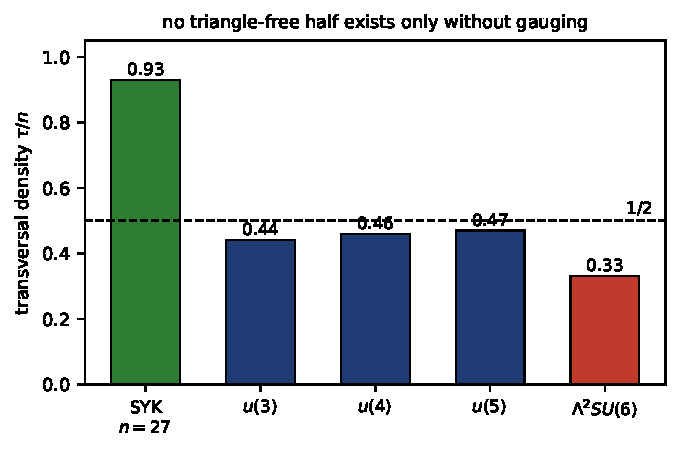
\includegraphics[width=0.47\textwidth]{report_figs/g_tau.pdf}
\caption{Transversal densities. SYK approaches $1$, since no triangle-free set exceeds $q-1$; gauge models sit
near $\frac12$, the positive-root half; two-index antisymmetric matter is worse still. This density governs
\eqref{eq:taubound}; the window itself is set by the symmetry class (\S\ref{sec:weyl}).}
\label{fig:tau}
\end{figure}

\begin{table}[t]\centering\small
\begin{tabular}{lrrrrl}
\toprule
$p$ & $\tau$ (closed form) & $\tau$ (ILP) & bound \eqref{eq:main} & measured $W$ & status\\
\midrule
1 & $N(N-1)/2$ & $3,6,10,15$ & $N+1$ & $N+1$ & tight\\
2 & $pN(N+1)/2-2N$ & $6,12,20$ & $2N+1$ & $2N+1$ & tight\\
3 & $pN(N+1)/2-2N$ & $5,12,22,35$ & $N+1$ & $N+1$ & tight\\
4 & $pN(N+1)/2-2N$ & $18$ & $1$ & $2N+1$ & valid, loose\\
\bottomrule
\end{tabular}
\caption{The transversal number and the resulting bound for single-trace $u(N)$. The closed form agrees with an
exact integer program in all $12$ cases tested ($p$ from $1$ to $4$, $N$ from $2$ to $6$).}
\label{tab:tau}
\end{table}

For SYK the same bound is vacuous, and instructively so. With generic couplings every $q$-subset is a triangle,
so $\alpha_{\rm SYK}=q-1$ and \eqref{eq:taubound} gives $W\ge2(q-1)-n+1$, negative for $n\ge2q-1$. The
transversal densities of Fig.~\ref{fig:tau} make the contrast concrete: $\tau/n=0.83,0.89,0.93$ for SYK at
$n=12,18,27$, against $0.44,0.46,0.47$ for $u(3),u(4),u(5)$ at $p=3$.

This bound is not tight in general, and the multi-trace couplings of \S\ref{sec:weyl} show the gap clearly:
they drive it to a vacuous value while leaving $W$ unchanged, exactly as expected once the window is known to
depend on the symmetry class rather than on the density. What \eqref{eq:cartan} contributes that
\S\ref{sec:rank} does not is a statement holding at every weight.

\section{Fortuity}\label{sec:fortuity}

For the single-matrix model the BPS states fill $r_*$, whose Young diagram is the staircase with $2N-2i$ boxes in
row $i$ and exactly $N-1$ rows. Going down in rank that diagram has too many rows to exist as a $U(M)$ irrep;
going up it is no longer the maximal-Casimir representation. The states exist at one rank only: they are
fortuitous rather than monotone. By \S\ref{sec:rank} the diagram of $\lambda^*$ has rows $p(2N-2i)$, the same
$N-1$ rows, so the argument generalises verbatim to all $p$. The difficulty is that our BPS states are not
confined to one irrep: at $N=3$, $p=3$ all thirteen irreps with $C_2\ge24$ carry them, each with window width
$4$. A statement about $\lambda^*$ alone cannot settle fortuity here, so we give a local argument instead.

\begin{figure}[t]\centering
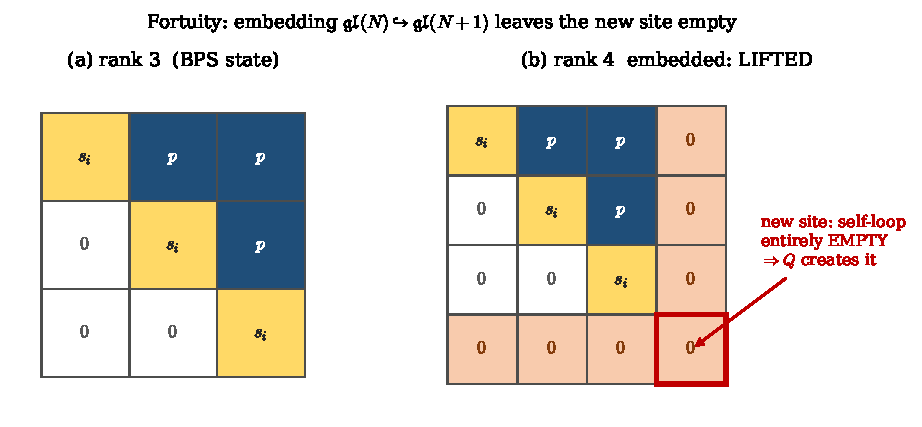
\includegraphics[width=0.85\textwidth]{report_figs/g_fortuity.pdf}
\caption{Embedding $\gl(N)\hookrightarrow\gl(N+1)$ as the upper-left block leaves every mode carrying the new
index unoccupied. The self-loop at the new site is then an entirely empty triangle, so $Q_{N+1}$ creates it and
the state is lifted.}
\label{fig:fortuity}
\end{figure}

Let $\iota$ embed $\gl(N)\hookrightarrow\gl(N+1)$ as the upper-left block. It is worth being careful about what
$\iota$ does and does not give, since it is \emph{not} a chain map: $\omega_{N+1}$ contains terms carrying the new
index that $\iota(\omega_N)$ does not, so $\omega_{N+1}\wedge\iota(m_S)\ne\iota(\omega_N\wedge m_S)$ and no map on
cohomology is induced. This is the observation of Tierz \cite{Tierz}, whose remedy is to compare ranks by the
projection $\pi_{M\to N}$ deleting every monomial that uses an index above $N$, which \emph{is} a chain map, and
to call a class fortuitous when it lies outside the image of the projections from all larger ranks.

What the triangle language supplies is the sharp local reason the inclusion fails, and it fails maximally. Under
the embedding every mode carrying the index $N+1$ is unoccupied, so the self-loop at the new site,
$T=\{\Psi^{a_1}_{N+1,N+1},\dots,\Psi^{a_q}_{N+1,N+1}\}$ with $q$ distinct flavours, satisfies $T\cap S=\varnothing$
for any embedded state $S$. A triangle disjoint from $S$ is precisely one that $Q$ can create, the Pauli blocking
of \S\ref{sec:everyweight} being absent, so $Q_{N+1}\,\iota(m_S)\ne0$: the embedded representative is not merely
unlifted, it is never closed. For $p<q$ the same holds for the sets $A_{\mathbf s}$ via the mixed loop
$i\to N+1\to j\to i$ with $i<j$, since the two edges through $N+1$ are new and hence empty while the return edge
$(j,i)$ is lower-triangular and hence empty. We verified this at $p=q=3$, where all $9$ BPS states of rank $2$ and
all $27$ of rank $3$ fail to be closed at the next rank, with the disjoint triangle exhibited in each case. So
the obstruction is uniform: it removes every BPS state at once, which is why no stabilisation map exists rather
than one that happens to vanish.

The two halves of this report rest on the same object, an empty triangle, and pull in opposite directions.
Enlarging the gauge group manufactures a fresh site whose self-loop is necessarily empty, which is what blocks
monotony and so produces fortuity; the same enlargement raises the rank, which by \S\ref{sec:rank} widens the
window and destroys concentration. The two properties one wants a fortuitous matrix model to have respond to the single available
structural knob with opposite signs, which may be why the combination has proved hard to realise.

\section{Status, and what is open}

\paragraph{Established.} The reduction \eqref{eq:wedge}; the index-loop restriction and the factorisation
\eqref{eq:kunneth} with the rank law \eqref{eq:ranklaw}; the bound $w_s\ge2$ and hence $W\ge r+1$ at the maximal
weight; the identification of SYK as the $r=1$ member, verified against the matrix code for $p$ from $4$ to $12$;
the vanishing of $\omega|_{\mathcal Z}$ whenever $-\mathrm{id}\in\Wg$, and the resulting classification of gauge
algebras; the closed and non-exact properties of critical states, \eqref{eq:taubound}, the positive-root
observation and \eqref{eq:cartan} for any reductive $\g$, with \eqref{eq:main} for $u(N)$; and the failure of
every embedded BPS state to be closed at the next rank.

\paragraph{Measured, not proved.} Three loadbearing statements are currently numerical. The floor
\eqref{eq:floor}, $\min_p w_s=q-1$, rests on scans at $q=3,5,7$ with $p\le13$. The growth of $W$ with $|\Wg|$ at
fixed mode count rests on five points and twenty coupling draws each. And the claim that the window is the same
in every irrep, not just at the maximal weight, rests on the complete spectra at $(p,N)=(1,3),(1,4),(2,3),(3,2)$
and the Casimir descents at $(3,3)$ and $(3,4)$. All cohomology is computed by exact integer linear algebra over
$\mathbb F_P$ with every rank confirmed against a second prime, cross-checked against the refined Witten index,
against exact diagonalisation at $N=2$, and against Chen's closed form at $p=1$.

\paragraph{Open.}
\begin{itemize}
\item \textbf{The Weyl growth, analytically.} The cleanest missing statement is a proof that a generic
$\Wg$-invariant $q$-form on $\mathbb C^p\otimes\h$ has window growing with $r$, which would turn
\S\ref{sec:weyl} from five measured points into the theorem the rank law deserves. A proof of \eqref{eq:floor}
would complete the $q$ dependence at the same time.
\item \textbf{An upper bound on $W$.} Everything here bounds the window from below, or computes it at the maximal
weight. The complementary statement, that the cohomology vanishes outside a band, equivalently that
$\omega\wedge$ is injective in low degrees, is verified in six models and four complete spectra but not
established. With it, the rank law would fix the window for every irrep and the no-go would become
spectrum-wide.
\item \textbf{$\su(N)$ away from the top.} The set $A_{\mathbf s}$ is not triangle-free there, since the Cartan
is $(N-1)$-dimensional and spread across sites, so Cartan triangles need not localise. The true transversal
numbers are $\tau=12,21,36$ for $N=3,4,5$ at $p=3$, giving bounds $1,4,1$ against measured widths $3,4,5$: valid,
tight only at $N=4$, vacuous at odd $N$. The factorisation \eqref{eq:kunneth} also fails, the profiles
$13,81,81,13$ and $15,258,486,258,15$ being non-binomial, although the rank law still predicts the widths
correctly.
\item \textbf{Macroscopic index.} Concentration is conditioned on macroscopic index, and the maximal irrep has
multiplicity $6^N=e^{1.8N}$, not $e^{O(N^2)}$. The descents reach $C_2=24$ at $N=3$ with Fock multiplicity
$110\,080$, the most macroscopic complex within reach, and the window does not close there. Reaching a genuinely
macroscopic complex needs a sparse exact rank routine.
\item \textbf{Chaos.} Nothing here bears on whether these models are chaotic. The three-flavour $H$ is not a
Casimir function, so a super-Schwarzian near-BPS spectrum remains possible without concentration.
\end{itemize}

\begin{thebibliography}{9}\small
\bibitem{Chen} Y.~Chen, \emph{Revisiting fortuity in matrix models}, 2025.
\bibitem{CCSY} C.~Chang, Y.~Chen, W.~Sia, S.~Yang, \emph{Fortuity in SYK models}, 2024.
\bibitem{ChangLin} C.~Chang, Y.~Lin, \emph{Words to describe fortuitous states}, 2024.
\bibitem{FGMS} W.~Fu, D.~Gaiotto, J.~Maldacena, S.~Sachdev, \emph{Supersymmetric SYK models},
Phys.\ Rev.\ D \textbf{95} (2017) 026009.
\bibitem{Tierz} M.~Tierz, \emph{BPS spectra of $\mathrm{Tr}[\Psi^p]$ matrix models for odd $p$},
arXiv:2604.27164, 2026.
\bibitem{TW} G.~Turiaci, E.~Witten, \emph{$\mathcal N=2$ JT supergravity and matrix models}, 2023.
\end{thebibliography}

\end{document}
